\subsection{Scalabilité}

\begin{frame}{Scalabilité}

    \begin{figure}[htb]
        \centering
        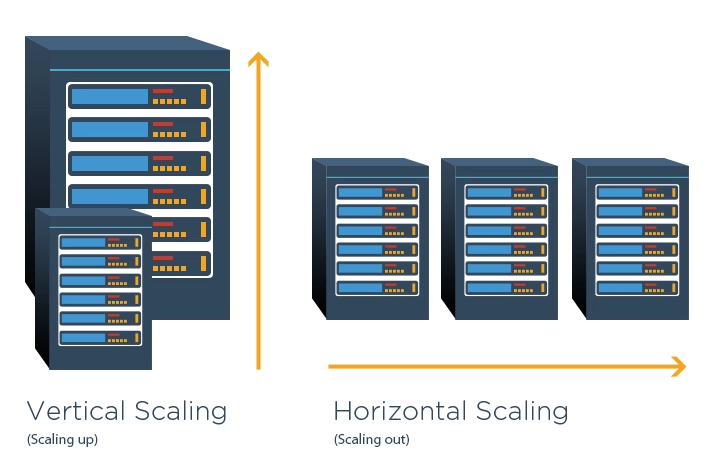
\includegraphics[width=0.9\textwidth]{img/horizontal-vs-vertical-scaling.png}
    \end{figure}

\end{frame}

\begin{frame}{Qu'est-ce que la scalabilité ?}

    Scalabilité horizontale : Ajout de machines pour augmenter la capacité de stockage et de traitement

    Scalabilité verticale : Ajout de ressources (CPU, RAM, Disque) sur une machine existante

    NoSQL databases are designed to scale out horizontally, meaning you can add more servers or nodes to the database cluster to handle increased data volume, traffic, or performance requirements. On the other hand, SQL databases often scale up vertically by adding more CPU, RAM, or storage capacity to a single server to handle increased demands.
\end{frame}

% ----------------------------------------------------------------------------------------------------------------------
% ----------------------------------------------------------------------------------------------------------------------
% ----------------------------------------------------------------------------------------------------------------------

\subsection{Partitionnement}

\begin{frame}{Qu'est-ce que le partitionnement ?}

    \begin{definitionbox}
        Le \textbf{partitionnement} (ou \textit{partitioning} en anglais) consiste à séparer les données en plusieurs \textit{chunks}.
    \end{definitionbox}

    \begin{figure}[htb]
        \begin{tikzpicture}
            \node[anchor=south west,scale=0.6,label=below:Data source] (singlefile) {\singlefile};

            \node[anchor=south west,scale=0.6,right=of singlefile,xshift=2cm,yshift=-0.5cm] (filechunck) {\filechunck};

            \draw [->, thick, draw=gray] ([yshift=-0.3cm]singlefile.east) -- node [above] {Chunking} (filechunck.west);
        \end{tikzpicture}
    \end{figure}

\end{frame}

\begin{frame}[standout]

    Partitionnement ou sharding ?

\end{frame}

\begin{frame}{Partitionnement vs sharding}

    \begin{definitionbox}
        Le \textbf{partitionnement} est une technique de division des données en plusieurs parties.
    \end{definitionbox}
    \pause
    \begin{definitionbox}
        Le \textbf{sharding} est une technique de distribution des données sur plusieurs n\oe{}uds.
    \end{definitionbox}

\end{frame}

\begin{frame}{Partitionnement vs sharding}
    \begin{figure}[htb]
        \resizebox{\textwidth}{!}{
        \begin{tikzpicture}
            \Large
            % Colors and styles
            \definecolor{lightblue}{RGB}{91,155,213}
            \definecolor{lightpurple}{RGB}{173,124,228}
            \definecolor{lightgray}{RGB}{239,240,241}

            \tikzstyle{db} = [shape border rotate=90, draw, thick, aspect=2, minimum height=8cm, minimum width=6cm, cylinder body fill=lightblue, cylinder end fill=lightgray]
            \tikzstyle{table cell} = [font=\scriptsize, draw=none]

            % Partitioning DB
            \node[db, cylinder, fill=lightgray, text centered] (partitioning) at (0,0) {};
            \node[above=of partitioning] {\textbf{PARTITIONING}};

            % Sharding DB
            \node[db, cylinder, text centered, label=below:\textbf{\Large Shard 1}, fill=lightpurple, right=of partitioning,xshift=3cm] (shard1) {};
            \node[db, cylinder, text centered, label=below:\textbf{\Large Shard 2}, fill=lightpurple, right=of shard1] (shard2) {};
            \node[above=of shard1,xshift=3.5cm] {\textbf{SHARDING}};

            \node[right=of partitioning,xshift=-0.1cm] {\textbf{VERSUS}};

            % Partitioning table
            \node[anchor=center,yshift=1.5cm] at (partitioning) (part1) {
                \begin{tabular}{|c|c|}
                    \hline
                    ID & Name \\ \hline
                    1 & Alice \\ \hline
                    2 & Bob \\ \hline
                    3 & Camille \\ \hline
                \end{tabular}
            };

            \node[anchor=center,below=of part1,yshift=1cm] (part2) {
                \begin{tabular}{|c|c|}
                    \hline
                    ID & Name \\ \hline
                    4 & Diane \\ \hline
                    5 & Elodie \\ \hline
                    6 & Fabrice \\ \hline
                \end{tabular}
            };

            % Sharding tables
            \node[anchor=center] at (shard1) {
                \begin{tabular}{|c|c|}
                    \hline
                    ID & Name\\ \hline
                    1 & Alice \\ \hline
                    2 & Bob \\ \hline
                    3 & Camille \\ \hline
                \end{tabular}
            };

            \node[anchor=center] at (shard2) {
                \begin{tabular}{|c|c|}
                    \hline
                    ID & Name\\ \hline
                    4 & Diane \\ \hline
                    5 & Elodie \\ \hline
                    6 & Fabrice \\ \hline
                \end{tabular}
            };

        \end{tikzpicture}
        }
    \end{figure}

\end{frame}

\begin{frame}{Différentes stratégies de partitionnement}
    \begin{columns}[onlytextwidth] % align columns
        \begin{column}{.48\textwidth}
            \begin{figure}[htb]
                \resizebox{\textwidth}{!}{
                \begin{tikzpicture}
                    % Include the file stack icon
                    \node[anchor=south west,scale=0.6,label=below:Data source] at (0,-1) (filechunck) {\filechunck};

                    \node[
                        database,ultra thick,database radius=1cm,
                        database segment height=0.5cm,
                        database top segment={draw=black,fill=customred},
                        database middle segment={draw=black,fill=customred},
                        database bottom segment={draw=black,fill=customred},
                        scale=0.6
                    ] at (5,2) (shard1) {};

                    \node[
                        database,ultra thick,database radius=1cm,
                        database segment height=0.5cm,
                        database top segment={draw=black,fill=customblue},
                        database middle segment={draw=black,fill=customblue},
                        database bottom segment={draw=black,fill=customblue},
                        scale=0.6
                    ] at (5,0) (shard2) {};

                    \node[
                        database,ultra thick,database radius=1cm,
                        database segment height=0.5cm,
                        database top segment={draw=black,fill=customgreen},
                        database middle segment={draw=black,fill=customgreen},
                        database bottom segment={draw=black,fill=customgreen},
                        scale=0.6
                    ] at (5,-2) (shard3) {};

                    % links
                    \draw [->, thick, draw=gray] (filechunck.east) -- node [above] {\textcolor{gray}{\bf ?}} (shard1.west);
                    \draw [->, thick, draw=gray] (filechunck.east) -- node [above] {\textcolor{gray}{\bf ?}} (shard2.west);
                    \draw [->, thick, draw=gray] (filechunck.east) -- node [above] {\textcolor{gray}{\bf ?}} (shard3.west);
                \end{tikzpicture}
                }
            \end{figure}
        \end{column}%
        \hfill%
        \begin{column}{.48\textwidth}
            \small
            \begin{itemize}
                \item Partitionnement par tourniquet
                \item Partitionnement par intervalle
                \item Partitionnement par clé/liste
                \item Partitionnement par hachage
            \end{itemize}
        \end{column}%
    \end{columns}
\end{frame}

\begin{frame}{Cas d'usage}

    Camille Lemoine est propriétaire d'une chaîne de trois restaurants situés à Paris, Londres et Dublin. Elle souhaite stocker les données de ses clients dans une base de données en fonction de ses différents restaurants.

    \begin{table}[]
        \begin{tabular}{|c|c|c|c|c|}
        \hline
        \rowcolor{lipstick}\color{white}\textbf{Identifiant} & \color{white}\textbf{Prénom} & \color{white}\textbf{Nom}  & \color{white}\textbf{Âge} & \color{white}\textbf{Ville}  \\\hline
        1000                 & Alice           & Dupont        & 30           & Paris \\
        1001                 & Bob             & Brown         & 39           & Londres \\
        1002                 & Charlie         & O'Brien       & 26           & Dublin \\
        1003                 & Daniel          & Doyle         & 42           & Dublin \\
        1004                 & Edna            & McCarthy      & 58           & Dublin \\
        1005                 & Fabienne        & Lenoir        & 66           & Paris \\
        1006                 & Gilles          & Morvan        & 71           & Paris \\
        \hline
        \end{tabular}
    \end{table}

    Elle vous demande de l'aider à choisir la meilleure stratégie de partitionnement pour stocker les données de ses clients en fonction de leur localisation.

\end{frame}

% ------------------------------------------------------------------------------------------------------------------------------------------------------------------------
%                                                                   Partitionnement par tourniquet
% ------------------------------------------------------------------------------------------------------------------------------------------------------------------------

\begin{frame}{Partitionnement par tourniquet}

    \begin{definitionbox}
        Le \textbf{partitionnement par tourniquet} (\textit{round-robin partitioning} en anglais) est une méthode de distribution des données où chaque enregistrement est successivement assigné à l'une des partitions disponibles de \textbf{manière cyclique}, assurant une répartition équilibrée de la charge
    \end{definitionbox}

    \pause

    \examplebox{
        \textbf{Comment assigner une donnée $i$ à un n\oe{}ud $n_j$ ?}

        La donnée située à l'index $i$ sera assignée au n\oe{}ud d'index $j$ noté $n_j$ avec \textit{$n_j$ = i mod n} et $n$ est le nombre de n\oe{}uds.
    }

\end{frame}


\begin{frame}{Partitionnement par tourniquet}
    \begin{figure}[htb]
        \resizebox{\textwidth}{!}{
        \begin{tikzpicture}

            \node[] at (-1.5,0) (users) {
                \begin{tabular}{|c|c|c|}
                    \hline
                    \textbf{ID} & \textbf{Prénom} & \textbf{Nom} \\ \hline
                    \only<2->{\rowcolor{customred!20}}1000 & Alice & Dupont \\
                    \only<3->{\rowcolor{customblue!20}}1001 & Bob & Brown \\
                    \only<4->{\rowcolor{customgreen!20}}1002 & Charlie & O'Brien \\
                    \only<5->{\rowcolor{customred!20}}1003 & Daniel & Doyle \\
                    \only<6->{\rowcolor{customblue!20}}1004 & Edna & McCarthy \\
                    \only<7->{\rowcolor{customgreen!20}}1005 & Fabienne & Lenoir \\
                    \only<8>{\rowcolor{customred!20}}1006 & Gilles & Morvan \\\hline
                \end{tabular}
                };

            \node[above=of users,text width=10cm,align=center] (question) {Comment partitionner par tourniquet\\ selon l'ID de l'utilisateur ?};
            \node[below=of users,text width=10cm,align=center] (remarque) {On considérera qu'un modulo 0 \\(ie 3 mod 3 = 0) correspond au n\oe{}ud 3.};

            \onslide<2>{\node[below=of users,yshift=-1.5cm] (alice) {Alice : user ID mod n = 1000 mod 3 = 1};}

            \node[
                database,ultra thick,database radius=1cm,
                database segment height=0.5cm,
                database top segment={draw=black,fill=customred},
                database middle segment={draw=black,fill=customred},
                database bottom segment={draw=black,fill=customred},
                scale=0.8,
                label=below:N\oe{}ud 1
            ] at (5,3) (shard1) {};

            \node[
                database,ultra thick,database radius=1cm,
                database segment height=0.5cm,
                database top segment={draw=black,fill=customblue},
                database middle segment={draw=black,fill=customblue},
                database bottom segment={draw=black,fill=customblue},
                scale=0.8,
                label=below:N\oe{}ud 2
            ] at (5,0) (shard2) {};

            \node[
                database,ultra thick,database radius=1cm,
                database segment height=0.5cm,
                database top segment={draw=black,fill=customgreen},
                database middle segment={draw=black,fill=customgreen},
                database bottom segment={draw=black,fill=customgreen},
                scale=0.8,
                label=below:N\oe{}ud 3
            ] at (5,-3) (shard3) {};

            \onslide<2-4>{\node[right=of shard1, xshift=0.1cm] (users1) {
                \begin{tabular}{|c|c|c|}
                    \hline
                    \textbf{ID} & \textbf{Prénom} & \textbf{Nom} \\
                    1000 & Alice & Dupont \\
                    \hline
                \end{tabular}
            };}

            \onslide<5-7>{\node[right=of shard1, xshift=0.1cm] (users1) {
                \begin{tabular}{|c|c|c|}
                    \hline
                    \textbf{ID} & \textbf{Prénom} & \textbf{Nom} \\
                    1000 & Alice & Dupont \\
                    1003 & Daniel  & Doyle \\
                    \hline
                \end{tabular}
            };}

            \onslide<8->{\node[right=of shard1, xshift=0.1cm] (users1) {
                \begin{tabular}{|c|c|c|}
                    \hline
                    \textbf{ID} & \textbf{Prénom} & \textbf{Nom} \\
                    1000 & Alice & Dupont \\
                    1003 & Daniel  & Doyle \\
                    1006 & Gilles & Morvan \\
                    \hline
                \end{tabular}
            };}

            \onslide<3-5>{\node[right=of shard2, xshift=0.1cm] (users2) {
                \begin{tabular}{|c|c|c|}
                    \hline
                    \textbf{ID} & \textbf{Prénom} & \textbf{Nom} \\
                    1001 & Bob  & Brown \\
                    \hline
                \end{tabular}
            };}

            \onslide<6->{\node[right=of shard2, xshift=0.1cm] (users2) {
                \begin{tabular}{|c|c|c|}
                    \hline
                    \textbf{ID} & \textbf{Prénom} & \textbf{Nom} \\
                    1001 & Bob  & Brown \\
                    1004 & Edna  & McCarthy \\
                    \hline
                \end{tabular}
            };}

            \onslide<4-6>{\node[right=of shard3, xshift=0.1cm] (users3) {
                \begin{tabular}{|c|c|c|}
                    \hline
                    \textbf{ID} & \textbf{Prénom} & \textbf{Nom} \\
                    1002 & Charlie & O'Brien \\
                    \hline
                \end{tabular}
            };}

            \onslide<7->{\node[right=of shard3, xshift=0.1cm] (users3) {
                \begin{tabular}{|c|c|c|}
                    \hline
                    \textbf{ID} & \textbf{Prénom} & \textbf{Nom} \\
                    1002 & Charlie & O'Brien \\
                    1005 & Fabienne & Lenoir \\
                    \hline
                \end{tabular}
            };}

            \onslide<2,5,8>{\draw [->, thick, draw=customred] (users) -- node [above,midway,align=center,sloped] {} (shard1);}
            \onslide<3,6>{\draw [->, thick, draw=customblue] (users) -- node [above,midway,align=center,sloped] {} (shard2);}
            \onslide<4,7>{\draw [->, thick, draw=customgreen] (users) -- node [above,midway,align=center,sloped] {} (shard3);}

        \end{tikzpicture}
        }
    \end{figure}
\end{frame}

\begin{frame}{Avantages et inconvénients du partitionnement par tourniquet}

    \prosbox{
        \textbf{Lecture} : Aucune partition spécifique n'est surchargée, car les données sont uniformément réparties.

        \textbf{Écriture} : Les écritures sont bien distribuées entre les partitions, évitant ainsi les goulots d'étranglement.
    }

    \pause

    \consbox{
        \textbf{Lecture} : Les requêtes qui nécessitent des recherches précises peuvent devoir scanner plusieurs partitions, augmentant ainsi le temps de lecture.

        \textbf{Écriture} : Il n'y a pas de regroupement logique des données, ce qui peut compliquer la gestion et l'accès à des ensembles de données liés.
    }

\end{frame}

% ------------------------------------------------------------------------------------------------------------------------------------------------------------------------
%                                                                   Partitionnement par intervalle
% ------------------------------------------------------------------------------------------------------------------------------------------------------------------------

\begin{frame}{Partitionnement par intervalle}

    \begin{definitionbox}
        Le \textbf{partitionnement par intervalle} ou également appelé partitionnement par plage (\textit{interval partitioning} en anglais) scinde les données en partitions basées sur des plages de valeurs spécifiques (par exemple, des plages de dates, de montants, etc.).
    \end{definitionbox}

    \pause

    \begin{noteblock}
        Le partitionnement par intervalle est souvent utilisé pour les données temporelles, où les enregistrements sont répartis en fonction de la date ou de l'heure de création.
    \end{noteblock}
\end{frame}

\begin{frame}{Partitionnement par intervalle}
    \begin{figure}[htb]
        \resizebox{\textwidth}{!}{
        \begin{tikzpicture}

            \node[] at (-1,0) (users) {
                \begin{tabular}{|c|c|c|c|}
                    \hline
                    \textbf{ID} & \textbf{Prénom} & \textbf{Nom} & \textbf{Âge} \\ \hline
                    \only<2->{\rowcolor{customred!20}}1000 & Alice & Dupont & 30 \\
                    \only<3->{\rowcolor{customred!20}}1001 & Bob  & Brown & 39 \\
                    \only<4->{\rowcolor{customred!20}}1002 & Charlie & O'Brien & 26 \\
                    \only<5->{\rowcolor{customblue!20}}1003 & Daniel  & Doyle & 42 \\
                    \only<6->{\rowcolor{customblue!20}}1004 & Edna  & McCarthy & 58 \\
                    \only<7->{\rowcolor{customblue!20}}1005 & Fabienne & Lenoir & 66 \\
                    \only<8>{\rowcolor{customgreen!20}}1006 & Gilles & Morvan & 71 \\\hline
                \end{tabular}
                };

            \node[above=of shard1, text width=14.5cm,xshift=-0.5cm,yshift=-0.5cm,align=center] (question) {Comment partitionner par intervalle selon l'âge de l'utilisateur avec les catégories d'âge suivantes : 20 à 39 ans, 40 à 69 ans et 70 ans et plus ?};

            \node[
                database,ultra thick,database radius=1cm,
                database segment height=0.5cm,
                database top segment={draw=black,fill=customred},
                database middle segment={draw=black,fill=customred},
                database bottom segment={draw=black,fill=customred},
                scale=0.8,
                label=below:N\oe{}ud 1
            ] at (5,3) (shard1) {};

            \node[
                database,ultra thick,database radius=1cm,
                database segment height=0.5cm,
                database top segment={draw=black,fill=customblue},
                database middle segment={draw=black,fill=customblue},
                database bottom segment={draw=black,fill=customblue},
                scale=0.8,
                label=below:N\oe{}ud 2
            ] at (5,0) (shard2) {};

            \node[
                database,ultra thick,database radius=1cm,
                database segment height=0.5cm,
                database top segment={draw=black,fill=customgreen},
                database middle segment={draw=black,fill=customgreen},
                database bottom segment={draw=black,fill=customgreen},
                scale=0.8,
                label=below:N\oe{}ud 3
            ] at (5,-3) (shard3) {};

            \onslide<2>{\node[right=of shard1, xshift=0.1cm] (users1) {
                \begin{tabular}{|c|c|c|c|}
                    \hline
                    \textbf{ID} & \textbf{Prénom} & \textbf{Nom} & \textbf{Âge} \\
                    1000 & Alice & Dupont & 30 \\
                    \hline
                \end{tabular}
            };}

            \onslide<3>{\node[right=of shard1, xshift=0.1cm] (users1) {
                \begin{tabular}{|c|c|c|c|}
                    \hline
                    \textbf{ID} & \textbf{Prénom} & \textbf{Nom} & \textbf{Âge} \\
                    1000 & Alice & Dupont & 30 \\
                    1001 & Bob  & Brown & 39 \\
                    \hline
                \end{tabular}
            };}

            \onslide<4->{\node[right=of shard1, xshift=0.1cm] (users1) {
                \begin{tabular}{|c|c|c|c|}
                    \hline
                    \textbf{ID} & \textbf{Prénom} & \textbf{Nom} & \textbf{Âge} \\
                    1000 & Alice & Dupont & 30 \\
                    1001 & Bob  & Brown & 39 \\
                    1002 & Charlie & O'Brien & 26 \\
                    \hline
                \end{tabular}
            };}

            \onslide<5>{\node[right=of shard2, xshift=0.1cm] (users2) {
                \begin{tabular}{|c|c|c|c|}
                    \hline
                    \textbf{ID} & \textbf{Prénom} & \textbf{Nom} & \textbf{Âge} \\
                    1003 & Daniel  & Doyle  & 42 \\
                    \hline
                \end{tabular}
            };}

            \onslide<6>{\node[right=of shard2, xshift=0.1cm] (users2) {
                \begin{tabular}{|c|c|c|c|}
                    \hline
                    \textbf{ID} & \textbf{Prénom} & \textbf{Nom} & \textbf{Âge} \\
                    1003 & Daniel  & Doyle  & 42 \\
                    1004 & Edna  & McCarthy & 58 \\
                    \hline
                \end{tabular}
            };}

            \onslide<7->{\node[right=of shard2, xshift=0.1cm] (users2) {
                \begin{tabular}{|c|c|c|c|}
                    \hline
                    \textbf{ID} & \textbf{Prénom} & \textbf{Nom} & \textbf{Âge} \\
                    1003 & Daniel  & Doyle   & 42 \\
                    1004 & Edna  & McCarthy  & 58 \\
                    1005 & Fabienne & Lenoir & 66 \\
                    \hline
                \end{tabular}
            };}

            \onslide<8->{\node[right=of shard3, xshift=0.1cm] (users3) {
                \begin{tabular}{|c|c|c|c|}
                    \hline
                    \textbf{ID} & \textbf{Prénom} & \textbf{Nom} & \textbf{Âge} \\
                    1006 & Gilles & Morvan & 71 \\
                    \hline
                \end{tabular}
            };}

            \onslide<2-4>{\draw [->, thick, draw=customred] (users) -- node [above,midway,align=center,sloped] {} (shard1);}
            \onslide<5-7>{\draw [->, thick, draw=customblue] (users) -- node [above,midway,align=center,sloped] {} (shard2);}
            \onslide<8>{\draw [->, thick, draw=customgreen] (users) -- node [above,midway,align=center,sloped] {} (shard3);}

        \end{tikzpicture}
        }
    \end{figure}
\end{frame}

\begin{frame}{Avantages et inconvénients du partitionnement par intervalle}

    \prosbox{
        \textbf{Lecture} : Efficace pour les requêtes qui filtrent sur une plage de valeurs spécifique, car elles accèdent uniquement à la partition pertinente.

        \textbf{Écriture} : Facile à comprendre et à gérer, particulièrement utile pour les données temporelles ou séquentielles.
    }

    \pause

    \consbox{
        \textbf{Lecture} : Les requêtes qui ne filtrent pas sur la colonne de partitionnement ou couvrent plusieurs plages peuvent être moins efficaces.

        \textbf{Écriture} : Les écritures peuvent se concentrer sur certaines partitions (par exemple, la partition la plus récente dans un partitionnement par date), créant un déséquilibre et un risque de surcharge de cette partition.
    }

\end{frame}

% ------------------------------------------------------------------------------------------------------------------------------------------------------------------------
%                                                                   Partitionnement par clé
% ------------------------------------------------------------------------------------------------------------------------------------------------------------------------

\begin{frame}{Partitionnement par clé}

    \begin{definitionbox}
        Le \textbf{partitionnement par clé (ou liste)} (\textit{key partitioning} ou \textit{list partitioning} en anglais) répartit les données en fonction de la valeur d'une ou plusieurs colonnes spécifiques, qui sont appelées les clés de partitionnement.
    \end{definitionbox}

    \pause

    \begin{noteblock}
        Le partitionnement par clé est souvent utilisé pour les données qui peuvent être regroupées en catégories distinctes, telles que les données géographiques, les catégories de produits, etc.
    \end{noteblock}
\end{frame}

% \begin{frame}{Partitionnement par clé}
%     \small

%     List partitioning is suitable for storing data whose columns contain a small number of enum values, and you often query and manage data based on these enum values.
%     For example, columns represent geographical locations, states, and categories. Each value in a column represents an independent category.
%      By partitioning data based on enum values, you can improve query performance and facilitate data management.

%     List partitioning is particularly useful for scenarios where a partition needs to include multiple values for each partitioning column.
%     For example, if a table includes the City column representing the city where an individual is from, and you often query and manage data by states and cities.
%     At table creation, you can use the City column as the partitioning column for List Partitioning and specify that data of various cities within the same state
%     are placed in one partition, for example PARTITION California VALUES IN ("Los Angeles", "San Francisco", "San Diego").
%     This method can accelerate queries based on states and cities while facilitating data management.

%     https://docs.starrocks.io/docs/table_design/list_partitioning

% \end{frame}

\begin{frame}{Partitionnement par clé}
    \begin{figure}[htb]
        \resizebox{\textwidth}{!}{
        \begin{tikzpicture}

            \node[] at (-1,0) (users) {
                \begin{tabular}{|c|c|c|c|}
                    \hline
                    \textbf{ID} & \textbf{Prénom} & \textbf{Nom}  & \textbf{Ville} \\ \hline
                    \only<2->{\rowcolor{customred!20}}1000 & Alice & Dupont & Paris \\
                    \only<3->{\rowcolor{customblue!20}}1001 & Bob & Brown & Londres \\
                    \only<4->{\rowcolor{customgreen!20}}1002 & Charlie & O'Brien & Dublin \\
                    \only<5->{\rowcolor{customgreen!20}}1003 & Daniel & Doyle & Dublin \\
                    \only<6->{\rowcolor{customgreen!20}}1004 & Edna & McCarthy & Dublin \\
                    \only<7->{\rowcolor{customred!20}}1005 & Fabienne & Lenoir & Paris \\
                    \only<8>{\rowcolor{customred!20}}1006 & Gilles & Morvan & Paris \\\hline
                \end{tabular}
                };

            \node[above=of shard1,align=center,xshift=-1cm,yshift=-0.6cm] (question) {Comment partitionner par clé selon la ville ?};

            \node[
                database,ultra thick,database radius=1cm,
                database segment height=0.5cm,
                database top segment={draw=black,fill=customred},
                database middle segment={draw=black,fill=customred},
                database bottom segment={draw=black,fill=customred},
                scale=0.8,
                label=below:N\oe{}ud 1
            ] at (5,3) (shard1) {};

            \node[
                database,ultra thick,database radius=1cm,
                database segment height=0.5cm,
                database top segment={draw=black,fill=customblue},
                database middle segment={draw=black,fill=customblue},
                database bottom segment={draw=black,fill=customblue},
                scale=0.8,
                label=below:N\oe{}ud 2
            ] at (5,0) (shard2) {};

            \node[
                database,ultra thick,database radius=1cm,
                database segment height=0.5cm,
                database top segment={draw=black,fill=customgreen},
                database middle segment={draw=black,fill=customgreen},
                database bottom segment={draw=black,fill=customgreen},
                scale=0.8,
                label=below:N\oe{}ud 3
            ] at (5,-3) (shard3) {};

            \onslide<2-6>{\node[right=of shard1, xshift=0.1cm] (users1) {
                \begin{tabular}{|c|c|c|}
                    \hline
                    \textbf{ID} & \textbf{Prénom} & \textbf{Nom} \\
                    1000 & Alice & Dupont \\
                    \hline
                \end{tabular}
            };}

            \onslide<7>{\node[right=of shard1, xshift=0.1cm] (users1) {
                \begin{tabular}{|c|c|c|}
                    \hline
                    \textbf{ID} & \textbf{Prénom} & \textbf{Nom} \\
                    1000 & Alice & Dupont \\
                    1005 & Fabienne & Lenoir \\
                    \hline
                \end{tabular}
            };}

            \onslide<8>{\node[right=of shard1, xshift=0.1cm] (users1) {
                \begin{tabular}{|c|c|c|}
                    \hline
                    \textbf{ID} & \textbf{Prénom} & \textbf{Nom} \\
                    1000 & Alice & Dupont \\
                    1005 & Fabienne & Lenoir \\
                    1006 & Gilles & Morvan \\
                    \hline
                \end{tabular}
            };}

            \onslide<3->{\node[right=of shard2, xshift=0.1cm] (users2) {
                \begin{tabular}{|c|c|c|}
                    \hline
                    \textbf{ID} & \textbf{Prénom} & \textbf{Nom} \\
                    1001 & Bob  & Brown \\
                    \hline
                \end{tabular}
            };}

            \onslide<4>{\node[right=of shard3, xshift=0.1cm] (users3) {
                \begin{tabular}{|c|c|c|}
                    \hline
                    \textbf{ID} & \textbf{Prénom} & \textbf{Nom} \\
                    1002 & Charlie & O'Brien \\
                    \hline
                \end{tabular}
            };}

            \onslide<5>{\node[right=of shard3, xshift=0.1cm] (users3) {
                \begin{tabular}{|c|c|c|}
                    \hline
                    \textbf{ID} & \textbf{Prénom} & \textbf{Nom} \\
                    1002 & Charlie & O'Brien \\
                    1003 & Daniel  & Doyle \\
                    \hline
                \end{tabular}
            };}

            \onslide<6->{\node[right=of shard3, xshift=0.1cm] (users3) {
                \begin{tabular}{|c|c|c|}
                    \hline
                    \textbf{ID} & \textbf{Prénom} & \textbf{Nom} \\
                    1002 & Charlie & O'Brien \\
                    1003 & Daniel  & Doyle \\
                    1004 & Edna  & McCarthy \\
                    \hline
                \end{tabular}
            };}

            \onslide<2,7,8>{\draw [->, thick, draw=customred] (users) -- node [above,midway,align=center,sloped] {} (shard1);}
            \onslide<3>{\draw [->, thick, draw=customblue] (users) -- node [above,midway,align=center,sloped] {} (shard2);}
            \onslide<4-6>{\draw [->, thick, draw=customgreen] (users) -- node [above,midway,align=center,sloped] {} (shard3);}

        \end{tikzpicture}
        }
    \end{figure}
\end{frame}

\begin{frame}{Avantages et inconvénients du partitionnement par clé}

    \prosbox{
        \textbf{Lecture} : Les requêtes qui filtrent sur la clé de partition sont rapides, car elles accèdent directement à la partition appropriée.

        \textbf{Écriture} : Les opérations d'écriture sont distribuées de manière équilibrée si la distribution des clés est uniforme, évitant ainsi les goulots d'étranglement.
    }

    \pause

    \consbox{
        \textbf{Lecture} : Si les requêtes ne filtrent pas sur la clé de partition, elles peuvent devoir parcourir plusieurs partitions, ce qui dégrade les performances.

        \textbf{Écriture} : Si les clés sont mal réparties (skewed distribution), certaines partitions peuvent être surchargées, entraînant des déséquilibres.
    }

\end{frame}

% ------------------------------------------------------------------------------------------------------------------------------------------------------------------------
%                                                                   Partitionnement par hachage
% ------------------------------------------------------------------------------------------------------------------------------------------------------------------------

\begin{frame}{Partitionnement par hachage}

    \begin{definitionbox}
        Le \textbf{partitionnement par hachage} (\textit{hash partitioning} en anglais) distribue les données en fonction du résultat d'une fonction de hachage appliquée à une ou plusieurs colonnes.
        $$f(x) = y$$
        avec $x$ la clé de partitionnement et $y$ le n\oe{}ud de destination.
    \end{definitionbox}

    \pause

    \begin{noteblock}
        Le partitionnement par hachage est souvent utilisé pour répartir uniformément les données et éviter les déséquilibres de charge. Les données sont réparties de manière aléatoire, mais déterministe.
    \end{noteblock}
\end{frame}

\begin{frame}{Partitionnement par hachage}
    \begin{figure}[htb]
        \resizebox{\textwidth}{!}{
        \begin{tikzpicture}

            \node[] at (-1,0) (users) {
                \begin{tabular}{|c|c|c|c|}
                    \hline
                    \textbf{ID} & \textbf{Prénom} & \textbf{Nom}  & \textbf{Hash} \\ \hline
                    \only<2->{\rowcolor{customblue!20}}1000 & Alice & Dupont & f(1000) = 2\\
                    \only<3->{\rowcolor{customred!20}}1001 & Bob& Brown  & f(1001) = 1\\
                    \only<4->{\rowcolor{customgreen!20}}1002 & Charlie & O'Brien & f(1002) = 3\\
                    \only<5->{\rowcolor{customgreen!20}}1003 & Daniel & Doyle & f(1003) = 3\\
                    \only<6->{\rowcolor{customred!20}}1004 & Edna & McCarthy & f(1004) = 1\\
                    \only<7->{\rowcolor{customblue!20}}1005 & Fabienne & Lenoir & f(1005) = 2\\
                    \only<8>{\rowcolor{customred!20}}1006 & Gilles & Morvan & f(1006) = 1\\ \hline
                \end{tabular}
                };

            \node[above=of shard1,text width=10cm,xshift=-1cm,yshift=-0.6cm] (question) {Comment partitionner par hachage selon l'ID de l'utilisateur ?};

            \node[
                database,ultra thick,database radius=1cm,
                database segment height=0.5cm,
                database top segment={draw=black,fill=customred},
                database middle segment={draw=black,fill=customred},
                database bottom segment={draw=black,fill=customred},
                scale=0.8,
                label=below:N\oe{}ud 1
            ] at (5,3) (shard1) {};

            \node[
                database,ultra thick,database radius=1cm,
                database segment height=0.5cm,
                database top segment={draw=black,fill=customblue},
                database middle segment={draw=black,fill=customblue},
                database bottom segment={draw=black,fill=customblue},
                scale=0.8,
                label=below:N\oe{}ud 2
            ] at (5,0) (shard2) {};

            \node[
                database,ultra thick,database radius=1cm,
                database segment height=0.5cm,
                database top segment={draw=black,fill=customgreen},
                database middle segment={draw=black,fill=customgreen},
                database bottom segment={draw=black,fill=customgreen},
                scale=0.8,
                label=below:N\oe{}ud 3
            ] at (5,-3) (shard3) {};

            \onslide<3-5>{\node[right=of shard1, xshift=0.1cm] (users1) {
                \begin{tabular}{|c|c|c|}
                    \hline
                    \textbf{ID} & \textbf{Prénom} & \textbf{Nom} \\
                    1001 & Bob  & Brown \\
                    \hline
                \end{tabular}
            };}

            \onslide<6-7>{\node[right=of shard1, xshift=0.1cm] (users1) {
                \begin{tabular}{|c|c|c|}
                    \hline
                    \textbf{ID} & \textbf{Prénom} & \textbf{Nom} \\
                    1001 & Bob  & Brown \\
                    1004 & Edna  & McCarthy \\
                    \hline
                \end{tabular}
            };}

            \onslide<8->{\node[right=of shard1, xshift=0.1cm] (users1) {
                \begin{tabular}{|c|c|c|}
                    \hline
                    \textbf{ID} & \textbf{Prénom} & \textbf{Nom} \\
                    1001 & Bob  & Brown \\
                    1004 & Edna  & McCarthy \\
                    1006 & Gilles & Morvan \\
                    \hline
                \end{tabular}
            };}

            \onslide<2-6>{\node[right=of shard2, xshift=0.1cm] (users2) {
                \begin{tabular}{|c|c|c|}
                    \hline
                    \textbf{ID} & \textbf{Prénom} & \textbf{Nom} \\
                    1000 & Alice & Dupont \\
                    \hline
                \end{tabular}
            };}

            \onslide<7->{\node[right=of shard2, xshift=0.1cm] (users2) {
                \begin{tabular}{|c|c|c|}
                    \hline
                    \textbf{ID} & \textbf{Prénom} & \textbf{Nom} \\
                    1000 & Alice & Dupont \\
                    1005 & Fabienne & Lenoir \\
                    \hline
                \end{tabular}
            };}

            \onslide<4>{\node[right=of shard3, xshift=0.1cm] (users2) {
                \begin{tabular}{|c|c|c|}
                    \hline
                    \textbf{ID} & \textbf{Prénom} & \textbf{Nom} \\
                    1002 & Charlie & O'Brien \\
                    \hline
                \end{tabular}
            };}

            \onslide<5->{\node[right=of shard3, xshift=0.1cm] (users3) {
                \begin{tabular}{|c|c|c|}
                    \hline
                    \textbf{ID} & \textbf{Prénom} & \textbf{Nom} \\
                    1002 & Charlie & O'Brien \\
                    1003 & Daniel  & Doyle \\
                    \hline
                \end{tabular}
            };}

            \onslide<3,6,8>{\draw [->, thick, draw=customred] (users) -- node [above,midway,align=center,sloped] {} (shard1);}
            \onslide<2,7>{\draw [->, thick, draw=customblue] (users) -- node [above,midway,align=center,sloped] {} (shard2);}
            \onslide<4-5>{\draw [->, thick, draw=customgreen] (users) -- node [above,midway,align=center,sloped] {} (shard3);}

        \end{tikzpicture}
        }
    \end{figure}
\end{frame}

\begin{frame}{Avantages et inconvénients du partitionnement par hachage}

    \prosbox{
        \textbf{Lecture} : Les requêtes qui utilisent la colonne de hachage sont rapides, car elles accèdent directement à la partition spécifique.

        \textbf{Écriture} : Les données sont réparties de manière uniforme, minimisant le risque de surcharge d'une partition.
    }

    \pause

    \consbox{
        \textbf{Lecture} : Les requêtes qui ne filtrent pas sur la colonne de hachage peuvent nécessiter un balayage de plusieurs partitions.

        \textbf{Écriture} : Le hachage peut rendre le regroupement logique des données plus difficile et compliquer les opérations de maintenance comme le rééquilibrage des partitions.
    }

\end{frame}

\begin{frame}{Comparatif des différentes stratégies de partitionnement}

    \begin{figure}[htb]
        \resizebox{\textwidth}{!}{
        \begin{tikzpicture}
            \node[label=below:Partitionnement par tourniquet] at (0,0) (tourniquet) {
                \begin{tabular}{|c|c|c|c|c|}
                    \hline
                    \textbf{Identifiant} & \textbf{Prénom} & \textbf{Nom}  & \textbf{Âge} & \textbf{Ville} \\\hline
                    \rowcolor{customred!20}1000 & Alice & Dupont & 30 & Paris \\
                    \rowcolor{customblue!20}1001 & Bob & Brown & 39 & Londres\\
                    \rowcolor{customgreen!20}1002 & Charlie & O'Brien & 26 & Dublin \\
                    \rowcolor{customred!20}1003 & Daniel & Doyle & 42 & Dublin \\
                    \rowcolor{customblue!20}1004 & Edna & McCarthy & 58 & Dublin \\
                    \rowcolor{customgreen!20}1005 & Fabienne & Lenoir & 66 & Paris \\
                    \rowcolor{customred!20}1006 & Gilles & Morvan & 71 & Paris \\\hline
                \end{tabular}
                };

            \node[label=below:Partitionnement par intervalle (âge),right=of tourniquet, xshift=0.1cm] (intervalle) {
                \begin{tabular}{|c|c|c|c|c|}
                    \hline
                    \textbf{Identifiant} & \textbf{Prénom} & \textbf{Nom}  & \textbf{Âge} & \textbf{Ville} \\\hline
                    \rowcolor{customred!20}1000 & Alice & Dupont & 30 & Paris \\
                    \rowcolor{customred!20}1001 & Bob & Brown & 39 & Londres\\
                    \rowcolor{customred!20}1002 & Charlie & O'Brien & 26 & Dublin \\
                    \rowcolor{customblue!20}1003 & Daniel & Doyle & 42 & Dublin \\
                    \rowcolor{customblue!20}1004 & Edna & McCarthy & 58 & Dublin \\
                    \rowcolor{customblue!20}1005 & Fabienne & Lenoir & 66 & Paris \\
                    \rowcolor{customgreen!20}1006 & Gilles & Morvan & 71 & Paris \\\hline
                \end{tabular}
                };

            \node[label=below:Partitionnement par clé (ville),below=of tourniquet, yshift=-0.1cm] (cle) {
                \begin{tabular}{|c|c|c|c|c|}
                    \hline
                    \textbf{Identifiant} & \textbf{Prénom} & \textbf{Nom}  & \textbf{Âge} & \textbf{Ville} \\\hline
                    \rowcolor{customred!20}1000 & Alice & Dupont & 30 & Paris \\
                    \rowcolor{customblue!20}1001 & Bob & Brown & 39 & Londres\\
                    \rowcolor{customgreen!20}1002 & Charlie & O'Brien & 26 & Dublin \\
                    \rowcolor{customgreen!20}1003 & Daniel & Doyle & 42 & Dublin \\
                    \rowcolor{customgreen!20}1004 & Edna & McCarthy & 58 & Dublin \\
                    \rowcolor{customred!20}1005 & Fabienne & Lenoir & 66 & Paris \\
                    \rowcolor{customred!20}1006 & Gilles & Morvan & 71 & Paris \\\hline
                \end{tabular}
                };

            \node[label=below:Partitionnement par hachage,right=of cle, xshift=0.1cm] (hachage) {
                \begin{tabular}{|c|c|c|c|c|}
                    \hline
                    \textbf{Identifiant} & \textbf{Prénom} & \textbf{Nom}  & \textbf{Âge} & \textbf{Ville} \\ \hline
                    \rowcolor{customblue!20}1000 & Alice & Dupont & 30 & Paris\\
                    \rowcolor{customred!20}1001 & Bob & Brown & 39 & Londres\\
                    \rowcolor{customgreen!20}1002 & Charlie & O'Brien & 26 & Dublin \\
                    \rowcolor{customgreen!20}1003 & Daniel & Doyle & 42 & Dublin \\
                    \rowcolor{customred!20}1004 & Edna & McCarthy & 58 & Dublin \\
                    \rowcolor{customblue!20}1005 & Fabienne & Lenoir & 66 & Paris \\
                    \rowcolor{customred!20}1006 & Gilles & Morvan & 71 & Paris \\\hline
                \end{tabular}
                };

        \end{tikzpicture}
        }
    \end{figure}

\end{frame}

\begin{frame}{Résumé des performances}

    \textbf{Lecture}
    \begin{itemize}
        \item \textbf{Meilleur} : Partitionnement par intervalle ou par clé (si les requêtes ciblent la clé ou l'intervalle).
        \item \textbf{Moins efficace} : Partitionnement par tourniquet ou par hachage pour des requêtes non ciblées.
    \end{itemize}

    \pause

    \textbf{Écriture}
    \begin{itemize}
        \item \textbf{Meilleur} : Partitionnement par hachage ou par tourniquet (distribution équilibrée des écritures).
        \item \textbf{Moins efficace} : Partitionnement par intervalle (risque de surcharge sur certaines partitions).
    \end{itemize}

    \pause

    Le choix de la stratégie dépend du type de requêtes majoritaires (lecture ou écriture), de la distribution des données, et des besoins spécifiques de l'application en termes de performance.
\end{frame}
